\chapter{Конструкторская часть}

\section{Схемы алгоритмов}

В данной части будут рассмотрены схемы алгоритмов нахождения расстояния Левенштейна и Дамерау-Левенштейна.
На рисунках 2.1-2.4 представлены данные алгоритмы.

\begin{figure}[h]
	\centering
	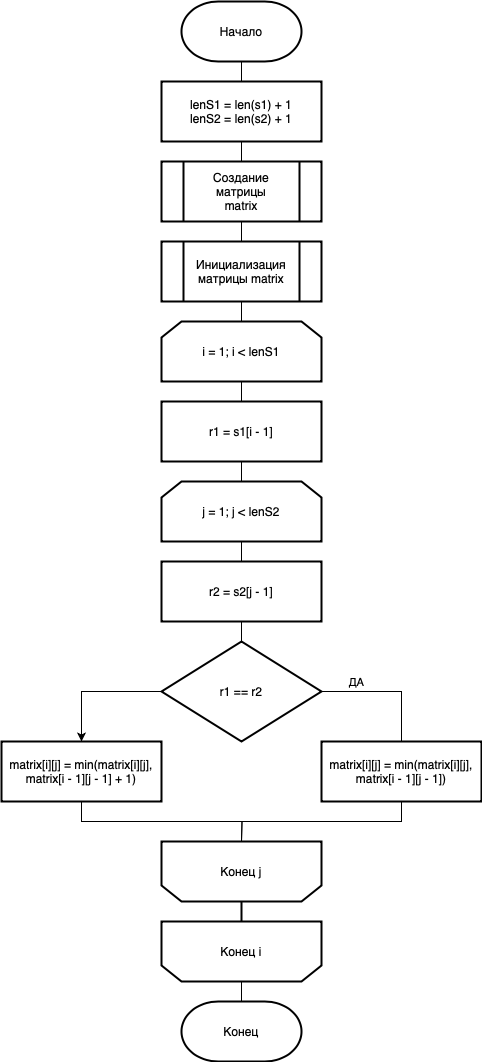
\includegraphics[width=0.5\linewidth]{img/L.jpg}
	\caption{Схема нерекурсивного алгоритма нахождения расстояния Левенштейна}
	\label{fig:mpr}
\end{figure}

\clearpage


\begin{figure}[h]
	\centering
	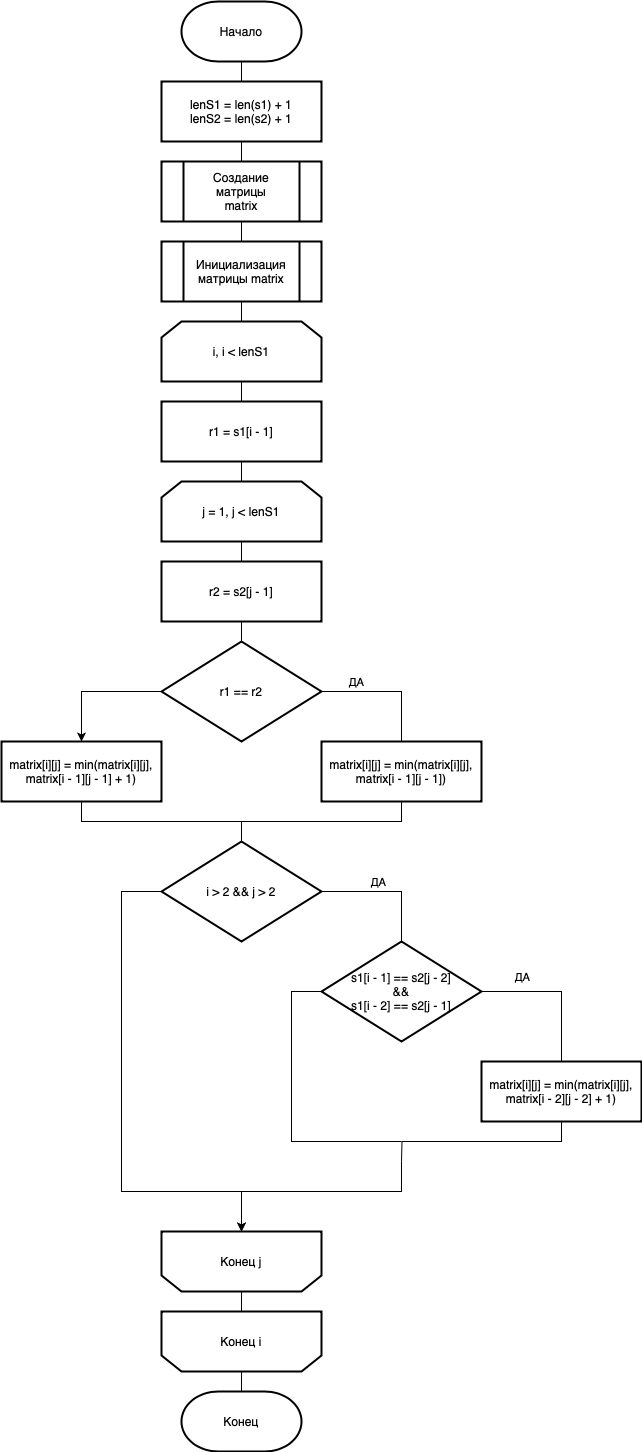
\includegraphics[width=0.65\linewidth]{img/DLM.jpg}
	\caption{Схема нерекурсивного алгоритма нахождения расстояния Левенштейна-Дамерау}
	\label{fig:mpr}
\end{figure}

\clearpage

\begin{figure}[h]
	\centering
	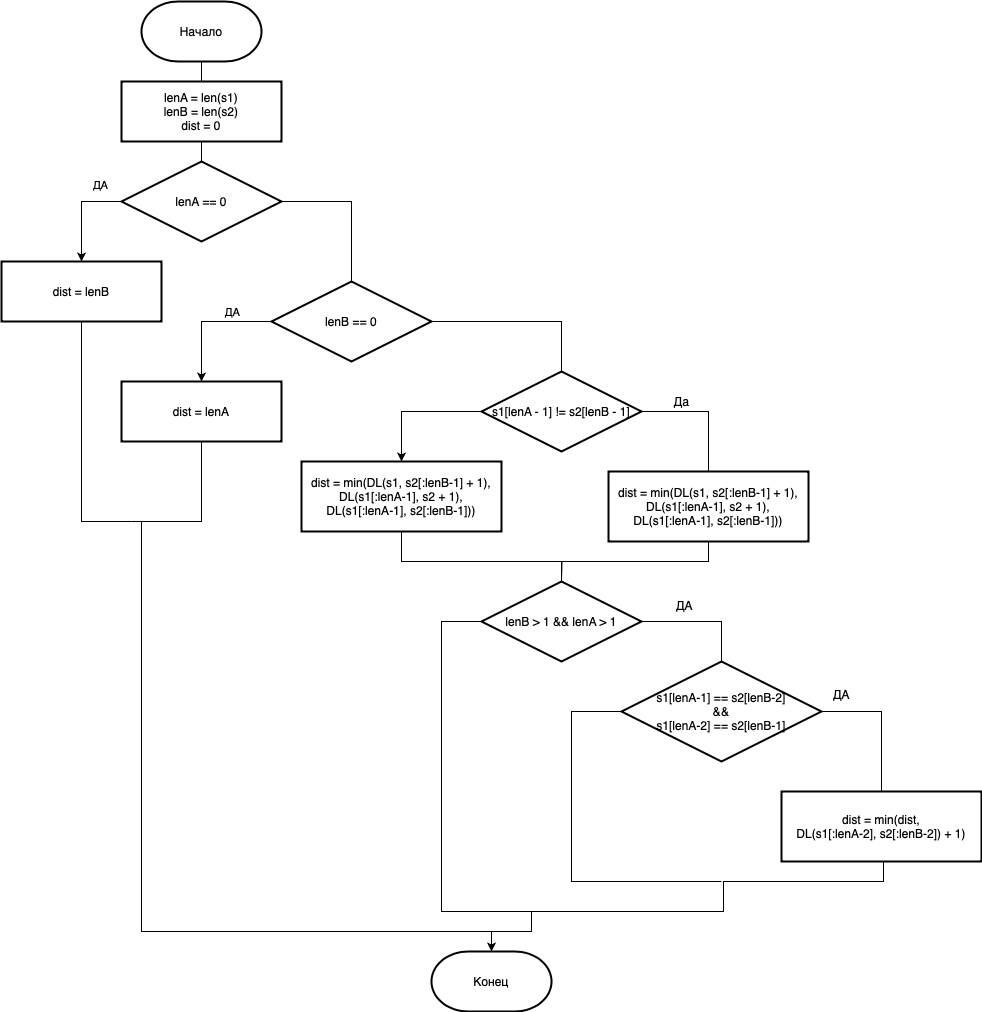
\includegraphics[width=1\linewidth]{img/DLR.jpg}
	\caption{Схема рекурсивного алгоритма нахождения расстояния Левенштейна-Дамерау}
	\label{fig:mpr}
\end{figure}

\clearpage

\begin{figure}[h]
	\centering
	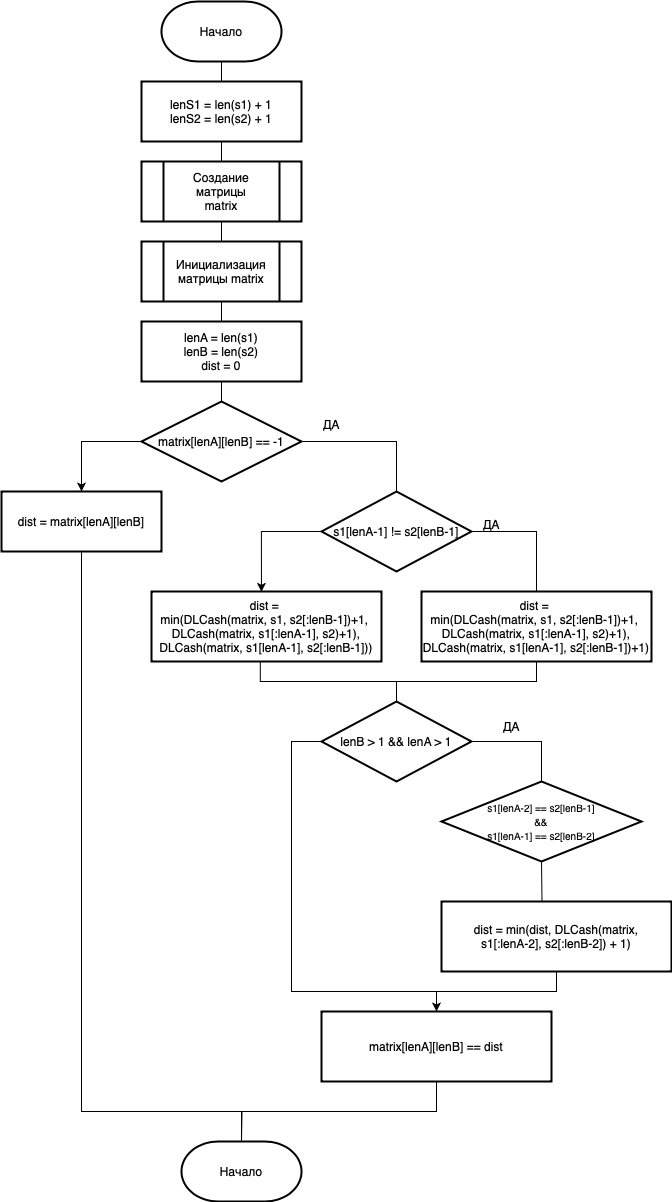
\includegraphics[width=0.8\linewidth]{img/DLC.jpg}
	\caption{Схема рекурсивного алгоритма нахождения расстояния Левенштейна-Дамерау с кешированием}
	\label{fig:mpr}
\end{figure}

\clearpage

\section{Вывод}
На основе теоретических даннных, полученных в аналитическом разделе были построены схемы исселедуемых алгоритмов.
